%
% File acl2021.tex
%
%% Based on the style files for EMNLP 2020, which were
%% Based on the style files for ACL 2020, which were
%% Based on the style files for ACL 2018, NAACL 2018/19, which were
%% Based on the style files for ACL-2015, with some improvements
%%  taken from the NAACL-2016 style
%% Based on the style files for ACL-2014, which were, in turn,
%% based on ACL-2013, ACL-2012, ACL-2011, ACL-2010, ACL-IJCNLP-2009,
%% EACL-2009, IJCNLP-2008...
%% Based on the style files for EACL 2006 by 
%%e.agirre@ehu.es or Sergi.Balari@uab.es
%% and that of ACL 08 by Joakim Nivre and Noah Smith

\documentclass[11pt,a4paper]{article}
\usepackage[hyperref]{acl2021}
\usepackage{times}
\usepackage{latexsym}
\renewcommand{\UrlFont}{\ttfamily\small}

% This is not strictly necessary, and may be commented out,
% but it will improve the layout of the manuscript,
% and will typically save some space.
\usepackage{microtype}

\usepackage{booktabs}
\usepackage{tabularx}
\newcolumntype{L}{>{\raggedright\arraybackslash}X}

\usepackage{graphicx}
\usepackage{placeins}


\aclfinalcopy % Uncomment this line for the final submission
%\def\aclpaperid{***} %  Enter the acl Paper ID here

%\setlength\titlebox{5cm}
% You can expand the titlebox if you need extra space
% to show all the authors. Please do not make the titlebox
% smaller than 5cm (the original size); we will check this
% in the camera-ready version and ask you to change it back.

\newcommand\BibTeX{B\textsc{ib}\TeX}

\title{Large-scale text pre-training helps with dialogue act recognition, but not without fine-tuning}


\author{
  Bill Noble  \and  Vladislav Maraev\\ 
  Centre for Linguistic Theory and Studies in Probability\\%
  Department of Philosophy, Linguistics and Theory of Science\\%
  University of Gothenburg\\
  \texttt{\{bill.noble,vladislav.maraev\}@gu.se} \\
  \\
}


\date{}

% We should make the comparison with other tasks where BERT representations work well AS IS (i.e., without finetuning) vs dialogue where 
% the pretraining is helpful, but not without finetuning
% Missing reference(s) from *SEM reviews
% Usefulness of in-domain pre-training for spoken dialogue
% Future work: dialogue act recognition is not enough to fully evaluate BERT for dialogue - other turn change prediction, intent classification, utterance segmentation and disfluency detection
%  

\begin{document}
\maketitle

\begin{abstract}
  We use dialogue act recognition (DAR)
  to investigate how well BERT represents utterances in dialogue,
  and how fine-tuning and large-scale pre-training contribute to its performance.
  We find that while both the standard BERT pre-training and pretraining on
  dialogue-like data are useful, task-specific fine-tuning is essential for good performance.
\end{abstract}

%INTRODUCTION

Large-scale neural language models trained on massive corpora of text data
have achieved state-of-the-art results on a variety of traditional NLP tasks.
Given that dialogue, especially spoken dialogue, 
is radically different from the kind of data these language models are pre-trained on,
it is uncertain whether they would be useful for dialogue-oriented tasks.
In the example from the Switchboard corpus, shown in Table~\ref{tab:example}, 
it is evident that the structure of dialogue is quite different from that of written text.
%even if one imagines a script for a movie or a play.
Not only is the internal structure of contributions different---%
with features such as disfluencies, repair, incomplete sentences, and various vocal sounds---%
but the sequential structure of the discourse is different as well.
%In dialogue, speakers take turns and switch perspectives.
%More generally, the way that utterances contribute to and cohere with the discourse
%is different from the relationship between sentences in a piece of written text.

In this paper, we investigate how well 
one such large-scale language model,
BERT \citep{devlinBERTPretrainingDeep2018}, 
represents utterances in dialogue.
We use dialogue act recognition (DAR) as a proxy task, 
since both the internal content and the sequential structure of utterances 
has bearing on this task 

\begin{table}
      \small
  \centering
  \begin{tabularx}{\linewidth}{llL}
    \toprule
    Speaker & DA & Utterance \\ \midrule
    A	&sd	& Well, I'm the kind of cook that I don't normally measure things,  \\
    A	&sd	& I just kind of throw them in \\
    A	&sd	& and, you know, I don't to the point of, you know, measuring down to the exact amount that they say.  \\
    B	&sv	& That means you're a real cook. \\
    A	&bd	& \texttt{<Laughter>} Oh, is that what it means.  \\
    A	&b	& Uh-huh.  \\
    A	&x	& \texttt{<Laughter>}.\\
             \bottomrule
  \end{tabularx}
  \caption{Example from the SWDA corpus (sw2827). Dialogue acts: \emph{sd}---Statement-non-opinion, \emph{sv}---Statement-opinion, \emph{bd}---Downplayer, \emph{b}---Backchannel, \emph{x}---Non-verbal. }
  \label{tab:example}
\end{table}

We have two main contributions.
First we find that while standard BERT pre-training is useful,
the model performs poorly without fine-tuning (\S\ref{sec:experiment2}).
Second, we find that further pre-training with data from the target domain shows promise for dialogue, 
but the results are mixed when pre-training with a larger corpus of dialogical data from outside the target domain (\S\ref{sec:experiment3}).

\section{Background}

\subsection{Dialogue Act Recognition}
The concept of a dialogue act is based on that of speech acts \citep{austinHowThingsWords2009}.
Breaking with classical semantic theory, speech act theory considers not only the propositional content of an utterance but also the actions, such as \emph{promising} or \emph{apologizing}, it carries out.
Dialogue acts extend the concept of the speech act, 
with a focus on the interactional nature of most speech.
%DAMSL \citep{coreCodingDialogsDAMSL1997} is an influential dialogue act tagging scheme 
%where dialogue acts are defined in part by whether they have a 
%\emph{forward-looking} function (are expecting a response) or 
%\emph{backward-looking} function (are in response to a previous utterance).

DAR is the task of labeling utterances with the dialogue act they perform 
from a given set of dialogue act tags.
As with other sequence labeling tasks in NLP, some notion of context is helpful in DAR.
One of the first performant machine learning models for DAR was a Hidden Markov Model 
that used various lexical and prosodic features as input \citep{stolckeDialogueActModeling2000}.
Most successful neural approaches also model some notion of context \citep[e.g.,][]{kalchbrennerRecurrentConvolutionalNeural2013,tranHierarchicalNeuralModel2017,botheContextbasedApproachDialogue2018,bothe2018conversational,zhao2018unified}.
%Following previous work, we model dialogue act sequences with an RNN over utterance representations,
%which are constructed by BERT.

\subsection{Transfer learning for NLP}
Transfer learning techniques allow a model trained on one task---often unsupervised---to be applied to another. 
Since annotating natural language data is expensive, there is a lot of interest in transfer learning for natural language processing. 
Word vectors \citep[e.g.,][]{mikolovDistributedRepresentationsWords2013,penningtonGloveGlobalVectors2014} are a ubiquitous example of transfer learning in NLP.
We note, however, that pre-trained word vectors are not always useful when applied to dialogue \cite{cerisaraEffectsUsingWord2vec2017}. 

%Recently, neural models trained on large datasets with various unsupervised tasks have found success creating sentence-level and contextual word representations. 
BERT, a multi-layer transformer model \citep{devlinBERTPretrainingDeep2018}, 
is pre-trained on two unsupervised tasks: 
\emph{masked token prediction} and \emph{next sentence prediction}.
In masked token prediction, some percentage of words are randomly replaced with a mask token.
The model is trained to predict the identity of the original token based on the context sentence.
In next sentence prediction, the model is given two sentences and trained to predict whether the second sentence follows the first in the original text or if it was randomly chosen from elsewhere in the corpus.
After pre-training, BERT can be applied to a supervised task by adding additional un-trained layers that take the hidden state of one or more of BERT's layers as input. 

There is some previous work applying BERT to dialogue.
\citet{baoPLATOPretrainedDialogue2019} and \citet{chenSemanticallyConditionedDialog2019a} both use BERT for dialogue generation tasks.
Similarly, \citet{vigComparisonTransferLearningApproaches2019} find BERT useful for selecting a response from a list of candidate responses in a dialogue.
\citet{mehriPretrainingMethodsDialog2019} evaluate BERT in various dialogue tasks including DAR, and find that a model incorporating BERT outperforms a baseline model.
Finally, \citet{chakravarty2019dialog} use BERT for dialogue act classification for a proprietary domain and achieves promising results, and \citet{ribeiro2019deep} surpass the previous state-of-the-art on generic dialogue act recognition for Switchboard and MRDA corpora. 
This paper aims to supplement the findings of previous work by investigating how much of 
BERT's success for dialogue tasks is due to its extensive pre-training and how much is due to 
task-specific fine-tuning.

% TODO: \citep{chakravarty2019dialog,ribeiro2019deep,yu2019midas}
% some motivation, maybe restate that we are not looking at the performance per say?



\paragraph{Fine-tuning vs.~further in-domain pre-training}
We experiment with the following two transfer learning strategies \citep{sunHowFineTuneBERT2019}:
\emph{further pre-training}, in which the model is trained in an un-supervised way, similar to its initial training scheme, but on data that is in-domain for the target task; and
\emph{single-task fine-tuning}, in which the model's encoder layers are optimized during training for the target task.

Whether or not the encoder model has undergone further in-domain pre-training, 
there remains a choice of whether to fine-tune during task training,
or simply extract features from the encoder model without training it (i.e., \emph{freezing}).
Freezing the encoder model is more efficient, 
since the gradient of the loss function need only be computed for the task-specific layers.
However, fine-tuning can lead to better performance since the encoding itself is adapted to the target task and domain.

\citet{petersTuneNotTune2019} investigate when it is best to fine-tune BERT for sentence classification tasks 
and find that when the target task is very similar to the pre-training task, 
fine-tuning provides less of a performance boost.
We note that there is some conceptual relationship between DAR and next sentence prediction, since the dialogue act constrains (or at least is predictive of) the dialogue act that follows it.
That said, the discourse strucutre of the encyclopedia and book data that makes up BERT's pre-training corpus
is probably quite different from that of natural dialogue.
%\citet{petersTuneNotTune2019} also consider whether the similarity of the pre-training and target domains may have similar consequences, but don't find an effect of domain similarly for the natural language inference tasks they tested on.
%As discussed in \S\ref{sec:data}, however, there are dramatic differences between written text and transcribed dialogue which may make fine-tuning necessary for DAR.


\section{Data}\label{sec:data}

\begin{table}[]
\centering
\small
\begin{tabular}{@{}ll@{}}
\toprule
\textbf{Switchboard}       & \textbf{AMI Corpus}                     \\ \midrule
Dyadic                     & Multi-party                             \\
Casual conversation        & Mock business meeting                   \\
Telephone                  & In-person \& video                      \\ \midrule
English                    & English                                 \\ 
Native speakers            & Native \& non-native speakers           \\ 
early '90s                 & 2000s                                   \\ \midrule
2200 conversations         & 171 meetings                            \\
  \hspace{1em} 1155 in SWDA               & \hspace{1em} 139 in AMI-DA                           \\
400k utterances             & 118k utterances                         \\
3M tokens                  & 1.2M tokens                             \\ \bottomrule
\end{tabular}
  \caption{Comparison between Switchboard and the AMI Meeting Corpus}
  \label{tab:corpora}
\end{table}

We perform experiments on the Switchboard Dialogue Act Corpus (SWDA), 
which is a subset of the larger Switchboard corpus, 
and the dialogue act-tagged portion of the AMI Meeting Corpus (AMI-DA). 
SWDA is tagged with a set of 220 dialogue act tags which, following  \citet{jurafskySwitchboardSWBDDAMSLShallowDiscourseFunction1997a}, we cluster into a smaller set of 42 tags.
AMI uses a smaller tagset of 16 dialogue acts \citep{Carletta2007}.
See Table~\ref{tab:corpora} for details.

% - DA distribution              % Vlad

\paragraph{Preprocessing}
% - Preprocessing: remove disfluencies, acronyms and speaker tokens in AMI, % Bill

We make an effort to normalize transcription conventions across SWDA and AMI.
We remove disfluency annotations and slashes from the end of utterances in SWDA.
In both corpora, acronyms are tokenized as individual letters. 
All utterances are lower-cased.

Utterances are tokenized with BERT's word piece tokenizer with a vocabulary of 30,000.
To this vocabulary we added five speaker tokens and prepend each utterance with a speaker 
token that uniquely identifies the corresponding speaker within that dialogue.

%\paragraph{Dialogue act grouping}
%For our corpora we also considered grouping the dialogue acts according to DAMSL coders manual \citep{jurafskySwitchboardSWBDDAMSLShallowDiscourseFunction1997a}: Forward-Communicative-Function (51.86\% of all DAs), Backwards-Communicative-Function (30.35\%), Other (9.04\%) and Communicative-Status (8.75\%).
%This allows the direct comparison between SWDA and AMI-DA.
%With respect to laughs, we observed an even distribution of them in the groups, except for the Communicative-Status group in the case of SWDA, because of the ``Nonverbal'' dialogue acts (see footnote~1).

\subsection{Pre-training corpora}

We also experiment with three unlabeled dialogue corpora, which we use to provide further pre-training for the BERT encoder.

The first two corpora are constructed from the same source as the dialogue act corpora.
We use the SWDA portion of the un-labeled Switchboard corpus (SWBD) and the entire AMI corpus (including the 32 dialogues with no human-annotated DA tags that are not included in the DAR training set).
In both cases, we exclude dialogues that are reserved for DAR testing.

We also experiment with a much larger a corpus (350M tokens) constructed from OpenSubtitles \citep{Lison2016}.
Because utterances are not labeled with speaker, we randomly assigned a speaker token to each utterance to maintain the format of the other dialogue corpora.

The pre-training corpora were prepared for the combined masked language modeling and next sentence (utterance) prediction task, as described by \citet{devlinBERTPretrainingDeep2018}.
For the smaller SWBD and AMI corpora, we generate and train on multiple epochs of data. Since there is randomness in the data preparation (e.g., which distractor sentences are chosen and which tokens are masked), we generate each training epoch separately.\footnote{For details, see the \href{https://github.com/huggingface/transformers/tree/1.1.0/examples/lm_finetuning}{finetuning example} from Hugging Face.}

\section{Model} % Bill

We use a simple neural architecture with two components: 
an encoder that vectorizes utterances (BERT), 
and single-layer RNN sequence model that takes the utterance representations as input.\footnote{
We have experimented with LSTM as the sequence model, but the accuracy was not significantly different compared to RNN. It can be explained by the absence of longer distance dependencies on this level of our model.}
%Since we are primarily interested in comparing different training and fine-tuning schemes for the utterance encoder, 
%we use a basic single-layer RNN as the sequence model in every configuration.
At each time step, the RNN takes the encoded utterance as input 
and its hidden state is passed to a linear layer with softmax over dialogue act tags.\footnote{
Other work has shown that DAR benefits from more sophisticated decoding, such as conditional random field \citep{chenDialogueActRecognition2017} and uncertainty propagation \citep{tranPreservingDistributionalInformation2017}.}

Conceptually, the encoded utterance represents the context-agnostic features of the utterance,
and the hidden state of the RNN represents the full discourse context.

%As a baseline utterance encoder, we use a word-level CNN with window sizes of 3, 4, and 5, each with 100 feature maps \citep{kimConvolutionalNeuralNetworks2014}. 
%The model uses 100-dimensional word embeddings, which are initialized with pre-trained gloVe vectors \citep{penningtonGloveGlobalVectors2014}.

For the BERT utterance encoder, we use the BERT\textsubscript{BASE} model with hidden size of 768 and 12 transformer layers and self-attention heads \citep[][\S3.1]{devlinBERTPretrainingDeep2018}.
In our implementation, we use the un-cased model provided by \citet{Wolf2020}.
The RNN has a hidden layer size of 100.

\subsection{Pre-training vs. fine-tuning} \label{sec:experiment2} % Bill
First, we analyze how pre-training affects BERT's performance as an utterance encoder.
To do so, we consider the performance of DAR models with three different utterance encoders:
\begin{itemize}\setlength\itemsep{-0.5em}
  \item \texttt{BERT-FT} -- pre-trained + DAR fine-tuning 
  \item \texttt{BERT-FZ} -- pre-trained, frozen during DAR
  \item \texttt{BERT-RI} -- random init. + DAR fine-tuning 
\end{itemize}

%\begin{table}[]
%\centering
%\begin{tabular}{@{}lrrrr@{}}
%\toprule
                           %& \multicolumn{2}{c}{SWDA}                          & \multicolumn{2}{c}{AMI-DA}                        \\ \midrule
                           %& \multicolumn{1}{c}{F1} & \multicolumn{1}{c}{acc.} & \multicolumn{1}{c}{F1} & \multicolumn{1}{c}{acc.} \\
%\texttt{BERT-FT} & 36.75           & 76.60                    & 43.42                  & 64.93                    \\
%\texttt{BERT-RI} & 32.18           & 73.80                    & 34.88                  & 60.89                    \\
%\texttt{BERT-FZ} & 7.75            & 55.61                    & 14.86                  & 48.34 \\ \midrule
    %Majority class    & 0.78  & 33.56 &  1.88 & 28.27      \\ \bottomrule
%\end{tabular}
  %\caption{Macro-average F1 and accuracy of BERT with standard pre-training and DAR fine-tuning (\texttt{BERT-FT}) vs.~the same model without pre-training (\texttt{BERT-RI}) and without fine-tuning (\texttt{BERT-FZ}).}
  %\label{tab:exp2}
%\end{table}

\texttt{BERT-FT} is more accurate than \texttt{BERT-RI} by several percentage points on both DA corpora,
suggesting that BERT's extensive pre-training does provide some useful information for DAR (Table~\ref{tab:results}).
This performance boost is much more pronounced in the macro-averaged F1 score,\footnote{We report both \emph{accuracy} (which is equal to micro-averaged or class-weighted F1) and \emph{macro-F1}, which is the unweighted average of the F1 scores of each class.}
which is explained by the fact that at the tag level, pre-training has a larger impact on less frequent tags
(see Figure 1 in the supplementary materials). 

%Comparing the performance of the fine-tuned encoder to that of the frozen model, 
%we see that pre-training alone is not enough.
The \texttt{BERT-FZ} performs very poorly compared to either \texttt{BERT-FT} or \texttt{BERT-RI}, however.
It is heavily biased towards the most frequent tags, which explains its especially poor macro-F1 score (Table~\ref{tab:results}).
In SWDA, for example, the model with a frozen encoder predicts one of the two most common tags (Statement-non-opinion or Acknowledge) 86\% of the time, whereas those two
tags account for only 51\% of the ground truth tags.
\texttt{BERT-FT} is much less biased; it predicts the two most common tags only 59\% of the time.

%These observations raise two questions.
%First, how does BERT's pre-training help with DAR? 
%And second, in what way are the representations learned by pre-trained BERT lacking?
%In other words, what is the contribution of fine-tuning?

%To help answer these questions, we compare performance of the above three models by dialogue act tag.

% TODO: add per dialogue act accuracy figures

\subsection{Impact of dialogue pre-training} \label{sec:experiment3} % Bill

Next, we assess the effect of additional dialogue pre-training on BERT's performance as an utterance encoder.\footnote{
In-domain pre-training is sometimes referred to as \textit{fine-tuning}, but we reserve that term for task-specific training on labeled data.}
\citet{sunHowFineTuneBERT2019} has reported that performing additional pre-training on unlabeled in-domain data improves performance on classification tasks. 
We want to see if BERT can benefit from pre-training on dialogue data, including from data outside the immediate target domain.

For each of the target corpora (SWDA and AMI-DA), we compare four different pre-training conditions: 
The in-domain corpus (\texttt{ID}), consisting of the AMI pre-training corpus for the AMI-DA model and the SWBD pre-traning corpus for the SWDA model; 
the cross-domain corpus (\texttt{CC}), consisting of both the AMI and SWBD pre-training corpora; 
and finally the OpenSubtitles corpus (\texttt{OS}).
As before, we experiment with both frozen and fine-tuned models at the task training stage.

We performed 10 epochs of pre-training on the in-domain models and 5 epochs of pre-training on the cross-domain models so that the total amount of training data was comparable. The OpenSubtitles models were trained for only one epoch but with much more total training time. 

In the fine-tuned condition, additional pre-training offers a modest boost in overall accuracy and a substantial boost to the macro-F1 scores, with the cross-domain corpus providing the largest boost.
In the frozen condition, only the very large OpenSubtitles corpus is helpful, suggesting that when adapting BERT to dialogue, the size of the corpus is more important than its quality or fidelity to the target domain.
Still, pre-training provides nowhere near the performance improvement achieved by fine-tuning on the target task.

\begin{table}[]
\begin{tabular}{@{}lrrrr@{}}
\toprule
           & \multicolumn{2}{c}{SWDA}                          & \multicolumn{2}{c}{AMI-DA}                        \\ \midrule
           & \multicolumn{1}{c}{F1} & \multicolumn{1}{c}{acc.} & \multicolumn{1}{c}{F1} & \multicolumn{1}{c}{acc.} \\
\texttt{BERT-FT}    & 36.75                  & 76.60                    & 43.42                  & 64.93                    \\
\texttt{BERT+ID-FT} & 43.63                  & 77.01                    & 46.70                  & \textbf{68.88}           \\
\texttt{BERT+CC-FT} & \textbf{47.78}         & \textbf{77.35}           & \textbf{48.86}         & 68.79                    \\ 
\texttt{BERT+OS-FT} & 41.42                  & 76.95                    & 48.65                  & 68.07                    \\ \midrule
\texttt{BERT-FZ}    &  7.75                  & 55.61           & 14.86                  & 48.34                    \\
\texttt{BERT+ID-FZ} &  6.46                  & 52.30                    & 14.48                  & 48.18                    \\
\texttt{BERT+CC-FZ} &  5.76                  & 51.14                    & 11.34                  & 40.48                    \\ 
\texttt{BERT+OS-FZ} &  \textbf{9.60}         & \textbf{57.67}           & \textbf{17.03}         & \textbf{51.03}           \\ \midrule
\texttt{BERT-RI} & 32.18           & 73.80                    & 34.88                  & 60.89                    \\ \midrule
    Majority class  & 0.78                   & 33.56                    &  1.88                  & 28.27      \\ 
    SotA            &    -                   & 83.1\footnotemark                     &     -                  &     -      \\ \bottomrule
\end{tabular}
\caption{Comparison of macro-F1 and accuracy with further in-domain (\texttt{ID}), cross-domain corpus (\texttt{CC}), and OpenSubtitles (\texttt{OS}) dialogue pre-training,
for the frozen (\texttt{FZ}) and fine-tuned (\texttt{FT}) conditions. \texttt{BERT-RI} uses a randomly initialized utterance encoder with no pre-training but with fine-tuning.}
  \label{tab:results}
\end{table}

\footnotetext{\citet{Kozareva2019}} 


\section{Discussion} 

A key aspiration of transfer learning is to expose the model to 
phenomena that are too infrequent to learn from labeled training data alone.
We show some evidence of that here.
Pre-trained \texttt{BERT-FT} performs better on infrequent dialogue acts than \texttt{BERT-RI}, 
suggesting it draws on the extensive pre-training to represent infrequent features of those utterances.
Indeed, a simple lexical probe supports this explanation: in utterances where the pre-trained model is correct and the randomly initialized model is not, the rarest word is 1.9 times rarer on average than is typical of corpus as a whole.

In spite of that, the representations learned through pre-training are simply not performant without
task-specific fine-tuning, suggesting that they are fundamentally lacking in information that is 
important for the dialogue context.
We should note that this is in stark contrast to many other non-dialogical semantic tasks,
where frozen BERT performs on par or \emph{better} than the fine-tuned model \citep{petersTuneNotTune2019}.

By performing additional pre-training on a large dialogue-like corpus (OpenSubtitles),
we were able to raise the performance of the frozen encoder by a small amount.
This deserves further investigation. 
\citet{baoPLATOPretrainedDialogue2019} find that further pre-training BERT on a large-scale Reddit and Twitter corpus is helpful for response selection, but given the unimpressive results with subtitles, it remains an open question how well the text chat and social media domains transfer to natural dialogue.

%This may also explain why all our best models perform better on SWDA: more of the information that interlocutors and dialogue act annotators rely on is present SWDA transcripts, whereas AMI-DA annotators receive clear instructions to pay attention to the videos \citep{GuidelinesDialogueAct2005}.
%This finding is consistent with that of \citet{bavelas2008gesturing} who demonstrate that in face-to-face dialogue, visual components, such as gestures, can convey information that is independent from what is conveyed by speech.

There is also abundant room to investigate how speech-related information, such as laughter, prosody, 
and disfluencies can be incorporated into a DAR model that uses pre-trained features.
\citet{stolckeDialogueActModeling2000} showed, for example, that dialogue acts can have specific prosodic manifestations that can be used to improve dialogue act classification.
Incorporating such information is crucial if models pre-trained on large-scale text corpora are to be adapted for use in dialogue applications.

%Another avenue for future research is what pre-training schemes are best for the dialogue domain.
%The training scheme for RoBERTa \citep{liuRoBERTaRobustlyOptimized2019}, for example, leaves out next sentence prediction as a pre-training task because they do not find that it improves performance on question answering and natural language inference tasks.
%The same may not be true of dialogue, however, where sequentiality is essential.

\bibliographystyle{acl_natbib}
\bibliography{acl2020}

%
% File acl2021.tex
%
%% Based on the style files for EMNLP 2020, which were
%% Based on the style files for ACL 2020, which were
%% Based on the style files for ACL 2018, NAACL 2018/19, which were
%% Based on the style files for ACL-2015, with some improvements
%%  taken from the NAACL-2016 style
%% Based on the style files for ACL-2014, which were, in turn,
%% based on ACL-2013, ACL-2012, ACL-2011, ACL-2010, ACL-IJCNLP-2009,
%% EACL-2009, IJCNLP-2008...
%% Based on the style files for EACL 2006 by 
%%e.agirre@ehu.es or Sergi.Balari@uab.es
%% and that of ACL 08 by Joakim Nivre and Noah Smith

\documentclass[11pt,a4paper]{article}
\usepackage[hyperref]{acl2021}
\usepackage{times}
\usepackage{latexsym}
\renewcommand{\UrlFont}{\ttfamily\small}

% This is not strictly necessary, and may be commented out,
% but it will improve the layout of the manuscript,
% and will typically save some space.
\usepackage{microtype}

\usepackage{booktabs}
\usepackage{tabularx}
\newcolumntype{L}{>{\raggedright\arraybackslash}X}

\usepackage{graphicx}
\usepackage{placeins}

%\aclfinalcopy % Uncomment this line for the final submission
%\def\aclpaperid{***} %  Enter the acl Paper ID here

%\setlength\titlebox{5cm}
% You can expand the titlebox if you need extra space
% to show all the authors. Please do not make the titlebox
% smaller than 5cm (the original size); we will check this
% in the camera-ready version and ask you to change it back.

\newcommand\BibTeX{B\textsc{ib}\TeX}

\title{Large-scale text pre-training helps with dialogue act recognition, but not without fine-tuning\\\textit{Appendix}}


\author{First Author \\
  Affiliation / Address line 1 \\
  Affiliation / Address line 2 \\
  Affiliation / Address line 3 \\
  \texttt{email@domain} \\\And
  Second Author \\
  Affiliation / Address line 1 \\
  Affiliation / Address line 2 \\
  Affiliation / Address line 3 \\
  \texttt{email@domain} \\}

\date{}

% We should make the comparison with other tasks where BERT representations work well AS IS (i.e., without finetuning) vs dialogue where 
% the pretraining is helpful, but not without finetuning
% Missing reference(s) from *SEM reviews
% Usefulness of in-domain pre-training for spoken dialogue
% Future work: dialogue act recognition is not enough to fully evaluate BERT for dialogue - other turn change prediction, intent classification, utterance segmentation and disfluency detection
%  

\begin{document}
\maketitle

%\appendix

\begin{figure*}[ht]
  \centering
  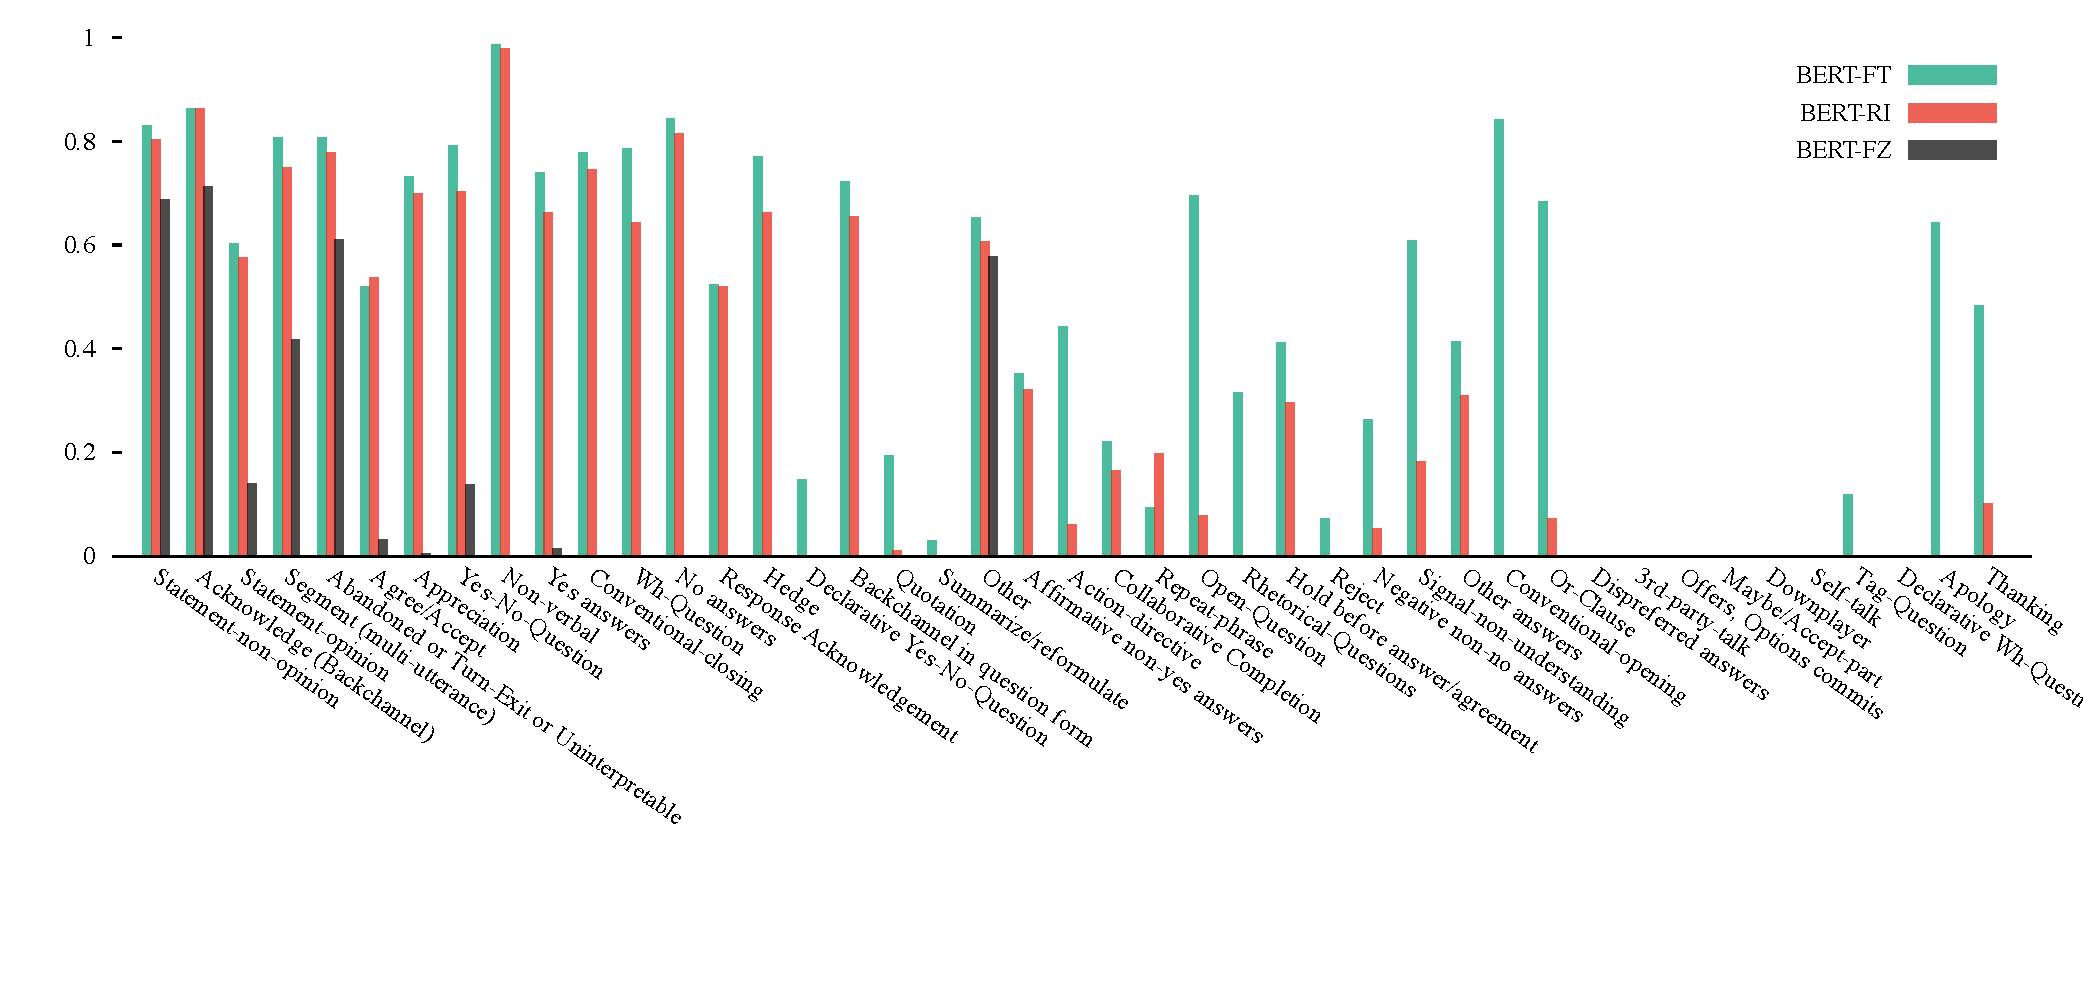
\includegraphics[width=\linewidth]{img/swda-brf.pdf}
  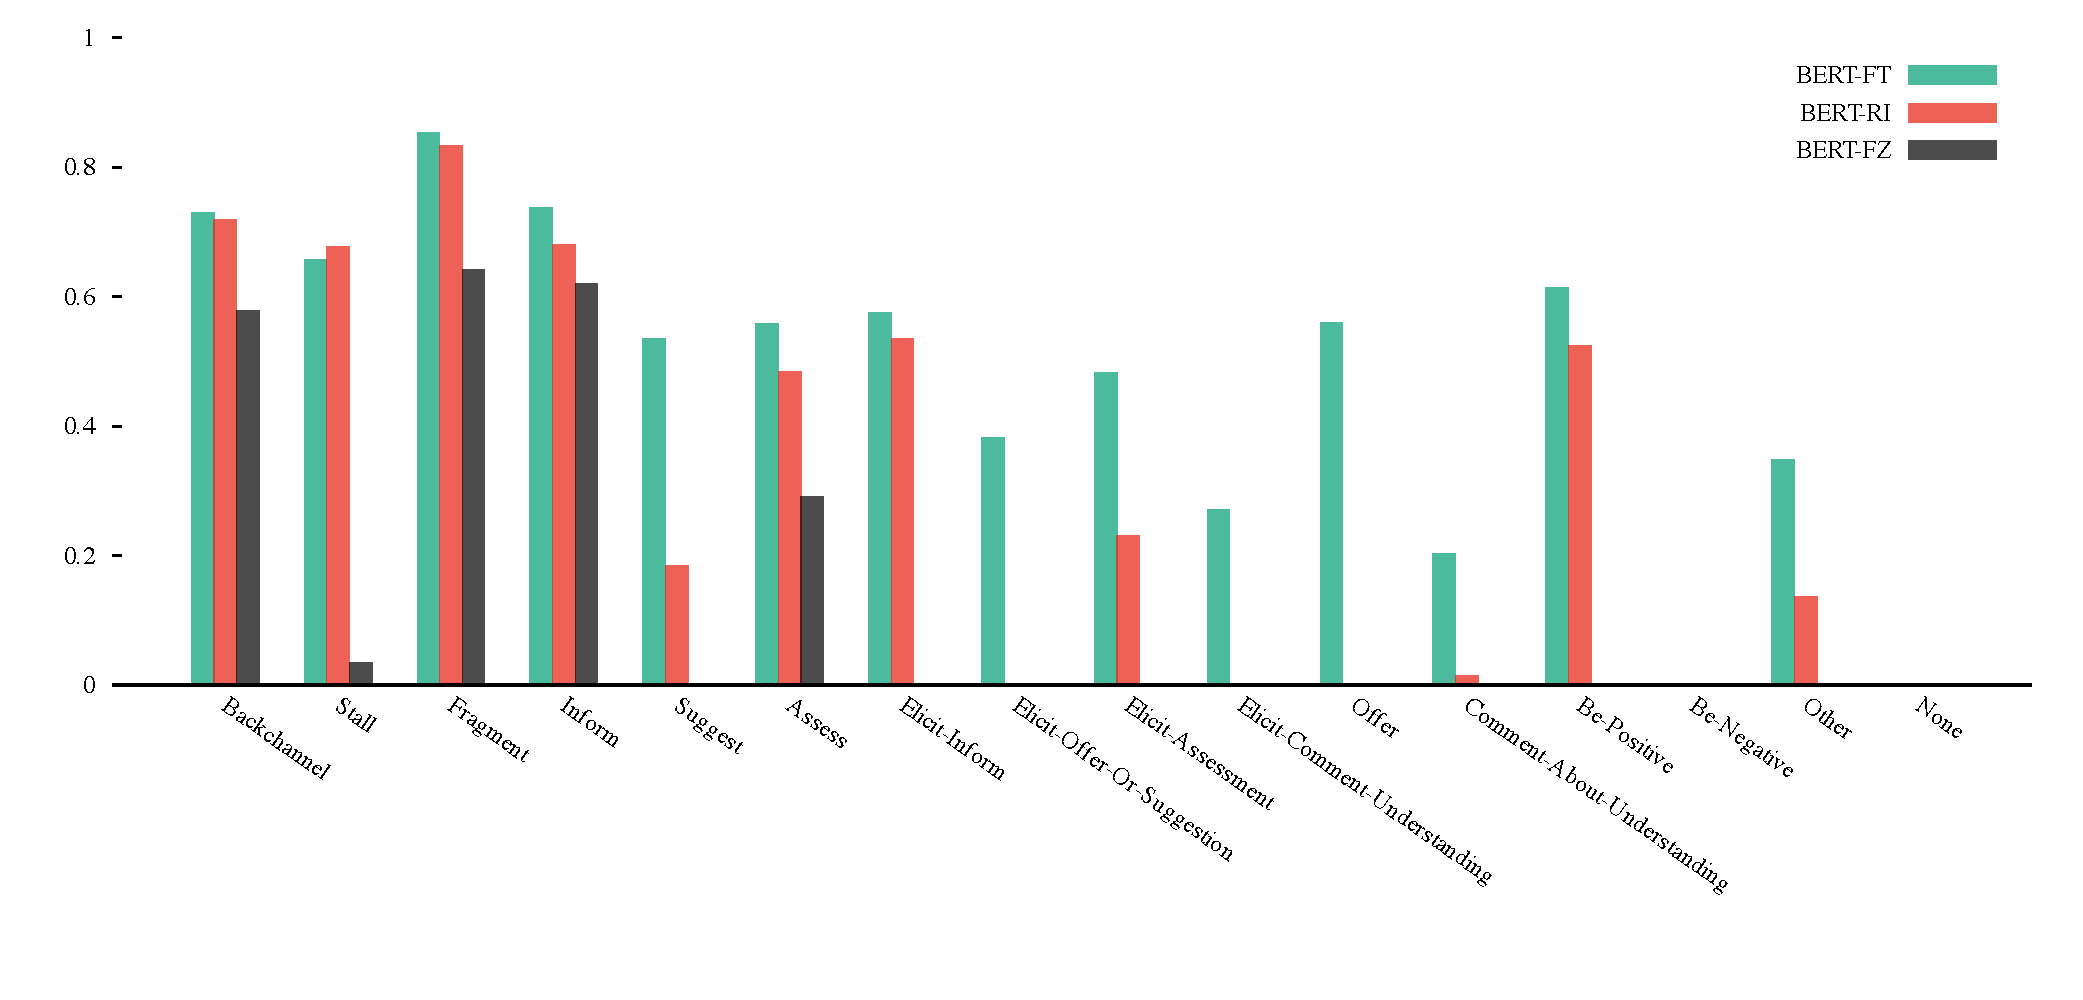
\includegraphics[width=\linewidth]{img/ami-brf.pdf}
  \caption{F1 scores by dialogue act for BERT with standard pre-training and DAR fine-tuning (\texttt{BERT-FT}) vs.~the same model without pre-training (\texttt{BERT-RI}) and without fine-tuning (\texttt{BERT-FZ}). Dialogue acts are ordered with the most common on the left.}
    \label{fig:f1-by-da}
  \end{figure*}

%\FloatBarrier
%\bibliographystyle{acl_natbib}
%\bibliography{acl2020}

\end{document}



\end{document}

